%%%%%%%%%%%%%%%%%%%%%%%%%%%%%%%%%%%%%%%%%%
% Capstone Project Handout
% LaTeX Template
% Version 1.0 (November 14, 2024)
% 
% Author:
% Matías Hoyl
% 
% License:
% CC BY-NC-SA 4.0 (https://creativecommons.org/licenses/by-nc-sa/4.0/)
%%%%%%%%%%%%%%%%%%%%%%%%%%%%%%%%%%%%%%%%%

%----------------------------------------------------------------------------------------
% PACKAGES AND OTHER DOCUMENT CONFIGURATIONS
%----------------------------------------------------------------------------------------

\documentclass[
    a4paper, % Paper size, use either a4paper or letterpaper
    10pt, % Default font size, can also use 11pt or 12pt
    twoside % Two side traditional mode where headers and footers change between odd and even pages
]{LTJournalArticle}

\usepackage{indentfirst} % Add this line to indent the first paragraph of each section
\usepackage{tabularx}
\usepackage{tcolorbox}
\tcbuselibrary{breakable, skins}
\usepackage{xcolor}
\usepackage{float} % Add this line to include the float package
\usepackage{enumitem} % Ensure this package is included
\usepackage{tcolorbox}
\tcbuselibrary{breakable,skins}
\usepackage{biblatex}
\addbibresource{references.bib} % BibLaTeX bibliography file

% Define slate color palette (keep your existing color definitions)
\definecolor{slate-50}{HTML}{F8FAFC}
\definecolor{slate-100}{HTML}{F1F5F9}
\definecolor{slate-200}{HTML}{E2E8F0}
\definecolor{slate-300}{HTML}{CBD5E1}
\definecolor{slate-400}{HTML}{94A3B8}
\definecolor{slate-500}{HTML}{64748B}
\definecolor{slate-600}{HTML}{475569}
\definecolor{slate-700}{HTML}{334155}
\definecolor{slate-800}{HTML}{1E293B}
\definecolor{slate-900}{HTML}{0F172A}

% Updated box definitions
\newtcolorbox{questionbox}[2][]{%
    enhanced,
    colback=slate-50,
    colframe=slate-400,
    boxrule=0.5pt,
    arc=4pt,
    title={#2},
    fonttitle=\bfseries\color{white},
    attach boxed title to top left={xshift=0.5cm,yshift=-\tcboxedtitleheight/2},
    boxed title style={
        colback=slate-400,
        colframe=slate-400,
        arc=2pt,
        boxrule=0pt,
    },
    top=12pt, % Increased top padding
    breakable,
    #1
}

\newtcolorbox{studentbox}[2][]{%
    enhanced,
    colback=slate-100,
    colframe=slate-500,
    boxrule=0.5pt,
    arc=4pt,
    title={#2},
    fonttitle=\bfseries\color{white},
    attach boxed title to top left={xshift=0.5cm,yshift=-\tcboxedtitleheight/2},
    boxed title style={
        colback=slate-500,
        colframe=slate-500,
        arc=2pt,
        boxrule=0pt,
    },
    top=12pt,
    breakable,
    #1
}

\newtcolorbox{llmbox}[2][]{%
    enhanced,
    colback=slate-200,
    colframe=slate-600,
    boxrule=0.5pt,
    arc=4pt,
    title={#2},
    fonttitle=\bfseries\color{white},
    attach boxed title to top left={xshift=0.5cm,yshift=-\tcboxedtitleheight/2},
    boxed title style={
        colback=slate-600,
        colframe=slate-600,
        arc=2pt,
        boxrule=0pt,
    },
    top=12pt,
    breakable,
    #1
}

%----------------------------------------------------------------------------------------
% TITLE SECTION
%----------------------------------------------------------------------------------------

\title{\Large Synthetic Students: Using Item Response Theory to Guide LLM-Based Answer Prediction}

% Authors are listed in a comma-separated list with superscript numbers indicating affiliations
\author{% 
    Matías Hoyl
}

% Remove the \date command to eliminate the date
% \date{}

\begin{document}

\maketitle

%----------------------------------------------------------------------------------------
% SECTION: OVERVIEW
%----------------------------------------------------------------------------------------
\section{Overview}
Educational assessment faces a significant challenge: developing and calibrating test items is expensive and time-consuming, requiring extensive student data. This project explores a novel solution by combining Item Response Theory (IRT) with Large Language Models (LLMs) to create "synthetic students" - AI systems that can simulate how real students would respond to test questions.

IRT provides robust, objective measurements of student abilities and question difficulty but requires substantial data for accurate calibration. LLMs, conversely, offer flexibility in understanding and generating human-like responses but may lack statistical rigor. By combining these approaches, we aim to leverage both IRT's psychometric precision and LLMs' adaptive capabilities to create more accurate student simulations.

If successful, this approach could streamline the test development process by using synthetic students for initial item calibration, reducing the need for extensive field testing while maintaining assessment quality.

%----------------------------------------------------------------------------------------
% SECTION: DATA
%----------------------------------------------------------------------------------------
\section{Data}
The data for this study is derived from Zapien, an adaptive educational platform in Chile, which includes 280,979 responses from around 5,000 students on mathematics questions. 

Key data preprocessing steps included the removal of missing values, filtering out students with fewer than 20 answers, and excluding unrealistic response times. 

Features engineered for richer context included average response timestamps, cumulative attempts per student, and skill levels for specific topics. 

%----------------------------------------------------------------------------------------
% SECTION: METHODS
%----------------------------------------------------------------------------------------
\section{Methods}

\subsection{Simulation Approach}
The simulation approach aimed to provide the LLM with enough context, including IRT ability, so it could find sufficient signal in that context and replicate how a student with those characteristics would respond to questions. We developed baseline and enhanced context scenarios to test this.

\subsubsection{Baseline Scenario}
In the baseline scenario, the LLM was given minimal context about the student—only their age and grade level—to see if it could realistically simulate student responses without much information.

\subsubsection{Enhanced Context Scenario}
In the enhanced scenario, the LLM was provided with a richer context, including historical performance metrics and a psychometric measure of student ability (\texttt{user\_level}) derived using IRT, ranging from -3 (low ability) to 3 (high ability). We developed an interpretative rubric to guide the LLM in simulating realistic student behavior based on these skill levels. The enriched prompt included prior successes, question difficulty, and other relevant academic details, helping the LLM generate more contextually accurate responses.

\subsection{Experimental Design}
Initial experiments used:
\begin{itemize}
    \item 20 representative questions balanced across grade levels
    \item Three LLM models: gpt-4o-mini, claude-3.5-haiku, gemini-1.5-flash
    \item 5 repetitions per test case to account for variability
\end{itemize}

\subsection{Metrics}
We used three metrics to evaluate the performance of the LLM:
\begin{itemize}
    \item \textbf{LLM Accuracy}: Checking if the response was correct
    \item \textbf{Response Alignment}: If the response matched the correctness of the student's actual answer
    \item \textbf{Exact Match}: If the LLM provided the identical answer as the student
\end{itemize}

%----------------------------------------------------------------------------------------
% SECTION: PRELIMINARY RESULTS
%----------------------------------------------------------------------------------------
\section{Preliminary Results}

The preliminary results showed that providing LLMs with enhanced contextual information improved their ability to simulate student responses more realistically. Accuracy rates were high in baseline scenarios, indicating a tendency towards correct answers. However, when richer context was provided, LLMs generated responses that were more aligned with the correct/incorrect nature of actual student answers, indicating improved behavioral simulation. 

\begin{figure}[H]
    \centering
    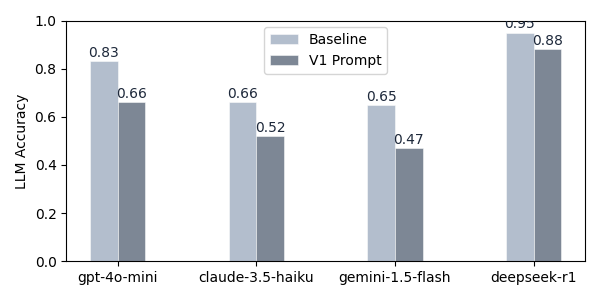
\includegraphics[width=\columnwidth]{../latex/images/llm_accuracy_comparison.png}
    \caption{LLM Accuracy: Baseline vs Enhanced Prompts}
    \label{fig:llm-accuracy}
\end{figure}

Response Alignment improved by up to 27\% with additional context, particularly for Anthropic's claude-3.5-haiku model. 

\begin{figure}[H]
    \centering
    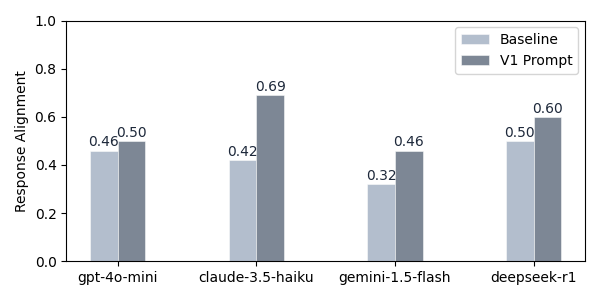
\includegraphics[width=\columnwidth]{../latex/images/response_alignment_comparison.png}
    \caption{Response Alignment: Baseline vs Enhanced Prompts}
    \label{fig:response-alignment}
\end{figure}

Exact Match rates showed modest improvements, reflecting the complexity of replicating specific incorrect answers.

\begin{figure}[H]
    \centering
    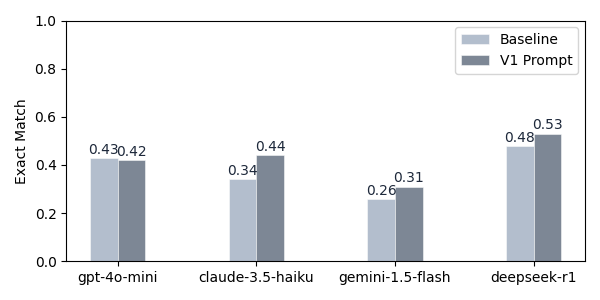
\includegraphics[width=\columnwidth]{../latex/images/exact_match_comparison.png}
    \caption{Exact Match Rates: Baseline vs Enhanced Prompts}
    \label{fig:exact-match}
\end{figure}

\subsection{LLM Reasoning Example}

\begin{questionbox}{Example Question}
    \textbf{Topic:} Multiplication of two-digit numbers \\
    \textbf{Subject:} Natural Numbers \\
    \textbf{Axis:} Arithmetic \\
    
    \textbf{Question:} What is the result of $31 \cdot 12$? \\
    
    \textbf{Options:}
    \begin{itemize}
        \item[(a)] 360
        \item[(b)] 651
        \item[(c)] 93
        \item[(d)] 372
        \item[(e)] None of the above
    \end{itemize}
    
    \textbf{Correct Answer:} b (not shown to the LLM)\\
    \textbf{Actual Student Answer:} c

\end{questionbox}

\begin{studentbox}{Student Characteristics}
    \begin{tabularx}{\textwidth}{Xr}
        \textbf{Age} & 12 \\
        \textbf{Skill Level} & -2.63 \\
        \textbf{Topic Previous Attempts} & 9 \\
        \textbf{Topic Success Rate} & 55\% \\
        \textbf{Subject Previous Attempts} & 34 \\
        \textbf{Subject Success Rate} & 64\% \\
        \textbf{Axis Previous Attempts} & 34 \\
        \textbf{Axis Success Rate} & 64\% \\
    \end{tabularx}
\end{studentbox}

\begin{llmbox}{Gemini 1.5 Flash Response}
    \textbf{Thinking Process:} Okay, so it's multiplication with two-digit numbers.  I'm not the best at this.  Remember those long multiplication problems we did last month?  Those were tricky, and I always got confused with carrying over numbers. I guess I can try to do it step-by-step. I'll first multiply 1 by 31, which is 31. Then, I'll multiply 2 by 31, but I'm not sure how to do that exactly... maybe it's 62?  Hmm, I think it's 62. Now I have to add those two together.  But how do I add them? It's like adding 31 and 62. Maybe the answer is around 90 or something? I see a lot of options, maybe 93? But I'm not sure.  I think it's 93, but I'm not completely sure.  I'm not very good at multiplying two-digit numbers, so I'm probably wrong.
    
    \textbf{Response:} c
    
    \textbf{Confidence:} 60
\end{llmbox}

%----------------------------------------------------------------------------------------
% SECTION: CHALLENGES AND FEEDBACK
%----------------------------------------------------------------------------------------
\section{Challenges}

The following are specific areas where I would appreciate feedback:

\begin{enumerate}
    \item \textbf{Statistical Significance of LLM Tests}: How can I ensure statistical significance in LLM experiments? What tests or methods should I use to validate my findings?
    \item \textbf{Monitoring Soft Metrics}: Besides accuracy and exact match, should I track metrics like "believability" of responses or reasoning consistency? How can I evaluate these qualitative aspects?
    \item \textbf{Literature Gaps}: Are there any studies similar to this work on simulating student behavior with LLMs?
\end{enumerate}

\end{document}
